\documentclass[tikz,border=8pt]{standalone}
% Shared look for every TikZ diagram. Load with \input{../../tools/tikz-style.tex}
\usepackage[T1]{fontenc}
\usepackage{lmodern}
\renewcommand{\sfdefault}{lmr}  % diagrams use the same serif as the text
\usetikzlibrary{arrows.meta, positioning, shapes.geometric, calc, fit, backgrounds}
\definecolor{cblue}{HTML}{4C78A8}
\definecolor{corange}{HTML}{F58518}
\definecolor{cgreen}{HTML}{54A24B}
\definecolor{cred}{HTML}{E45756}
\definecolor{cpurple}{HTML}{B279A2}
\definecolor{cgrey}{HTML}{6B6B6B}
\tikzset{
  every picture/.style={font=\sffamily, line width=1.2pt},
  box/.style={draw=#1, fill=#1!12, rounded corners=4pt, align=center, inner sep=7pt, minimum height=1.1cm},
  box/.default=cgrey,
  arrow/.style={-{Stealth[length=3mm]}, draw=cgrey, line width=1.4pt},
  title/.style={font=\sffamily\bfseries\Large},
  note/.style={font=\sffamily\small, text=cgrey, align=center},
}
\AtBeginDocument{\hyphenpenalty=10000 \exhyphenpenalty=10000}

\begin{document}
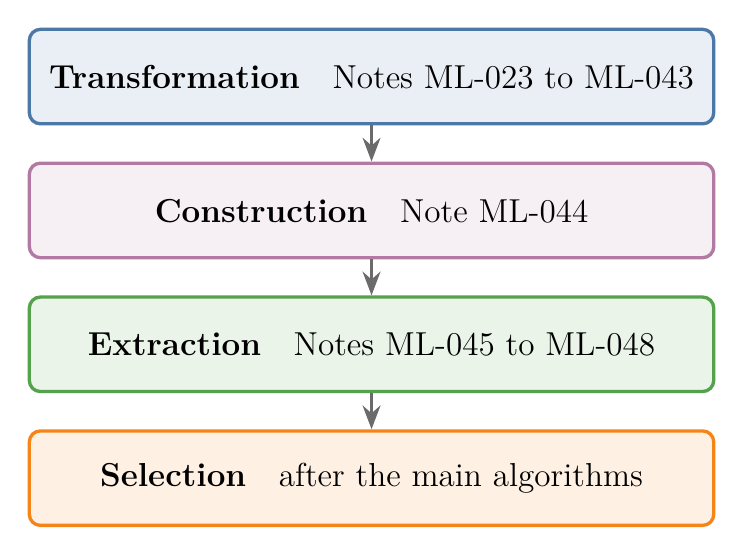
\begin{tikzpicture}[every node/.append style={font=\sffamily\large}]
\tikzset{note/.style={font=\sffamily\large, text=cgrey, align=center}}
  \tikzset{blk/.style={box=#1, minimum height=1.2cm, font=\sffamily\large}}
  \node[blk=cblue, text width=8.2cm] (t) at (0,0) {\textbf{Transformation}\quad Notes ML-023 to ML-043};
  \node[blk=cpurple, text width=8.2cm] (c) at (0,-1.7) {\textbf{Construction}\quad Note ML-044};
  \node[blk=cgreen, text width=8.2cm] (e) at (0,-3.4) {\textbf{Extraction}\quad Notes ML-045 to ML-048};
  \node[blk=corange, text width=8.2cm] (s) at (0,-5.1) {\textbf{Selection}\quad after the main algorithms};
  \draw[arrow] (t) -- (c); \draw[arrow] (c) -- (e); \draw[arrow] (e) -- (s);
\end{tikzpicture}
\end{document}
